%In Figure 2~\ref{process} the three steps of the conduction phase. As can be seen, in Step 1, we identified primary studies in the digital libraries. The digital libraries Scopus has returned more primary studies than the others(262), i.e., IEEE, ACM and Springer have returned 215, 202 and 127, respectively. Possibly, this came about because this digital library indexes studies of others libraries, such as IEEE and Springer. Summing up, we have gotten 802 primary studies in the Step 1. In the Step 2 we have selected the primary studies by means of reading the titles and abstracts and the application of the inclusion and exclusion criteria. As a result, we have gotten a total of 124 primary studies that were read entirely, so the upshot obtained in the Step 3 were 62. Among these 62 primary studies we have identified 18 mining techniques for crosscutting concern. Therefore, each included primary study was assigned to one or more techniques.
%
%\begin{figure}[!h]
%\centering
%  % Requires \usepackage{graphicx}
%  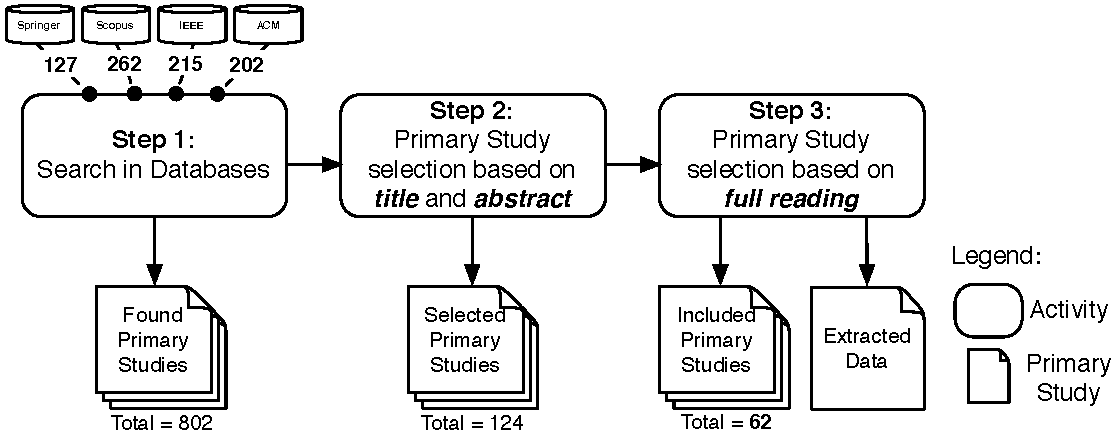
\includegraphics[scale=0.4]{figuras/process_conducted}
%\caption{Papers retrieved from each electronic database, total of candidate studies and the final set.}
%\label{process}
%\end{figure} 

Firstly we identified primary studies in the following digital libraries: IEEE, ACM, Scopus, Web of Science and Engeneering Village. We applied the search string given in Figure~\ref{search_string}. %Thus, an overview of results acquired from these digital libraries is depicted in Table~\ref{result_digital}.

%\begin{table}[!h]
%\centering
%\caption{Overview of search results.}
%\begin{tabular}{|c|c|}
%\hline 
%\cellcolor{gray}Digital Libraries & \cellcolor{gray}Number\tabularnewline
%\hline 
%\hline 
%Scopus & 150\tabularnewline
%\hline 
%ACM & 51\tabularnewline
%\hline 
%Engeneering Village & 30\tabularnewline
%\hline 
%Web of Science & 17\tabularnewline
%\hline 
%IEEE & 11\tabularnewline
%\hline 
%\cellcolor{gray!25}Total & \cellcolor{gray!25}259\tabularnewline
%\hline 
%\cellcolor{gray!25}Candidates & \cellcolor{gray!25}82\tabularnewline
%\hline 
%\cellcolor{gray!25}Final set & \cellcolor{gray!25}30\tabularnewline
%\hline 
%\end{tabular}
%\label{result_digital}
%\end{table} 


%As can be seen in Table~\ref{result_digital} 
The digital libraries Scopus returned more primary studies than the others (150), ACM, Engeneering Village, Web of Science and IEEE returned 51, 30, 17 and 11, respectively. Possibly, this occurred because Scopus indexes studies of others libraries, such as IEEE and ACM. Summarizing, we obtained 259 primary studies. After performing automatic search, we excluded the duplicate publications. If a primary study was found in more than once, we selected the most recent and detailed version of the paper. Afterwards, we selected the primary studies by reading the titles and abstracts and the application of the inclusion and exclusion criteria. At this stage, we also narrowed down the categories of publications to some extent by excluding non-peer reviewed publications, in order to ensure a level of quality as well as to avoid redundancy in contributions. As a result, we acquired a total of 82 primary studies that were read entirely, so the upshot obtained were 30 studies. A total of 229 studies were excluded either due to their limited relevance or meeting one of the other exclusion criterions.

We applied the classification schemes proposed by Petersen et al.~\cite{Petersen:2008:SMS:2227115.2227123} and classified the publications into categories from three perspectives, as follows: (\textit{i}) focus area, (\textit{ii}) contribution type and (\textit{iii}) research type. We chose this classification scheme because it is highly used in secondary study, i.e., papers which describe systematic review~\cite{Durelli:2013:SRM:2480362.2480567}.% and systematic mapping~\cite{Mehmood:2013:AMC:2400747.2401009}. %Although, this classification schemes has been proposed to be applied during a systematic mapping, we claim that it can be used during the systematic review process as well. 
 Thus, the aforementioned categories were adapted to specifics of our systematic study. The resultant classification schemes are as follows:

\subsubsection{Focus Area}

We used the keywording method described in~\cite{Petersen:2008:SMS:2227115.2227123} to identify the focus area of the identified studies. As result we got four ones - a brief description of each focus area follows: (\textit{i}) \textbf{Approaches to modernize legacy systems to another platform/architecture (SOA, change programming language, web $2.0$, mobile, etc):} This focus area is related to primary studies which describe process, method or approach that uses ADM and its metamodels to modernize legacy systems either to another platform  or architecture; (\textit{ii}) \textbf{Business Knowledge Extraction:} Describes primaries studies which address process, method or approach to extract business process of a legacy system; (\textit{iii}) \textbf{Extension of ADM's Metamodels:} This focus area represents primary studies which report an approach, method or process to extend one of the ADM's metamodels; and (\textit{iv}) \textbf{Applicability:} This category includes papers that mainly focus on reporting evidence related to applying ADM and its metamodels in practice. In other words, papers which enable researchers and practitioners to get a better understanding and utilization of ADM and its metamodels.

%\begin{itemize}

%\item \textbf{Approaches to modernize legacy systems to another platform/architecture (SOA, change programming language, web $2.0$, mobile, etc):} This focus area is related to primary studies which describe process, method or approach that uses ADM and its metamodels to modernize legacy systems either to another platform  or architecture.

%\item \textbf{Business Knowledge Extraction:} Describes primaries studies which address process, method or approach to extract business process of a legacy system.

%\item \textbf{Extension of ADM's Metamodels:} This focus area represents primary studies which report an approach, method or process to extend one of the ADM's metamodels, e.g., extension of KDM, SMM, ASTM, etc. 

%\item \textbf{Applicability:} This category includes papers that mainly focus on reporting evidence related to applying ADM and its metamodels in practice. In other words, papers which enable researchers and practitioners to get a better understanding of ADM and its metamodels, e.g., papers that show how to use the metamodels (KDM, SMM and ASTM) and provide a basis for the further research, etc.

%\end{itemize}


\subsubsection{Contribution Type}


During the reading of the primary studies was possible to identify a set of contribution types related to ADM and their metamodels. We identified five contribution types: (\textit{i}) \textbf{Tool:} This contribution type refers to the primary studies that focus on providing tools to support the modernization of legacy system by using ADM and its metamodels, i.e., either in the form of a prototype or a tool that can be integrated with existing environments; (\textit{ii}) \textbf{Process:} Similarly, it refers to contributions which specifically describe a process to assist the modernization of legacy system by means of ADM and its metamodels; (\textit{iii}) \textbf{Model Transformation:} It refers to contributions which describe transformation among ADM's metamodels, e.g., primary studies that describe the use of language transformation such as Query/Views/Transformations (QVT)\footnote{http://www.omg.org/spec/QVT/1.1/} or ATL Transformation Language (ATL)\footnote{www.eclipse.org/atl/}; (\textit{iv}) \textbf{Metamodel:} This contribution type describes primary studies which create or extend the ADM's metamodels to deal with a specific problem, for instance, providing a KDM light-weight extension in order to either represent the aspect oriented paradigm or supports a component-oriented decomposition; and (\textit{v}) \textbf{Metrics:} This type of contributions focus on proposing or applying metrics to effectiveness of ADM and its metamodels.

%\begin{itemize}

%\item \textbf{Tool:} This contribution type refers to the primary studies found that focus on providing tool in order to support the modernization of legacy system by using ADM and its metamodels, i.e., either in the form of a prototype or a tool that can be integrated with existing environment.



%\item \textbf{Process:} Similarly, it refers to contributions which specifically describe a process to assist the modernization of legacy system by means of ADM and its metamodels.

%\item \textbf{Model Transformation:} It refers to contributions which specifically describe transformation among ADM's metamodels, e.g., primary studies that describe the use of language transformation such as either Query/Views/Transformations (QVT)\footnote{http://www.omg.org/spec/QVT/1.1/} or ATL Transformation Language (ATL)\footnote{www.eclipse.org/atl/}. 

%\item \textbf{Metamodel:} This contribution type describes primary studies which either created or extended the ADM's metamodels to deal with a specific problem, for instance, providing a KDM light-weight extension in order to either represent the aspect oriented paradigm or supports a component-oriented decomposition.


%\item \textbf{Metrics:} This is type of contributions focus on proposing or applying metrics to effectiveness of ADM and its metamodels

%\end{itemize}

\subsubsection{Research Type}\label{research_type}

The research type reflects the research approach used in the primary study. We used and adapted the scheme proposed by Wieringa et al~\cite{Wieringa:2005:REP:1107677.1107683} herein. A brief description of research types are as follows: (\textit{i}) \textbf{Validation research:} The main purpose of validation research is to examine a solution proposal that has not yet been practically applied. Validation research is conducted in a systematic way and may present any of these: prototypes, math analysis, etc; (\textit{ii}) \textbf{Evaluation research:} In contrast to validation research, evaluation research aims at examining a solution that has already been practically applied. It investigates the practical implementation of solution and usually presents results using field studies, experiments, or case studies, etc; (\textit{iii}) \textbf{Conceptual proposal:} A conceptual proposal presents an arrangement to perceive things that already exist, in a novel way. However it does not precisely solve a particular problem. Conceptual proposals may include taxonomies, theoretical frameworks, etc; (\textit{iv}) \textbf{Experience paper:} An experience paper reports on personal experience of the author from one or more real life projects. It usually elaborates on what was accomplished in the project as well as how it was actually done; and (\textit{v}) \textbf{Opinion paper:} Opinion papers report on personal opinion of the author on suitability or unsuitability of a specific technique or tool. Similarly, these are sometimes used to share personal opinion describing as to how some technique or tool should have been developed, etc.

%\begin{itemize}
 
%\item \textbf{Validation research:} The main purpose of validation research is to examine a solution proposal that has not yet been practically applied. Validation research is conducted in a systematic way and may present any of these: prototypes,mathematical analysis, etc. 

%\item \textbf{Evaluation research:} In contrast to validation research, evaluation research aims at examining a solution that has already been practically applied. It investigates the practical implementation of solution and usually presents results using field studies, experiments, or case studies, etc.

%\item \textbf{Conceptual proposal:} A conceptual proposal presents an arrangement to see things that already exist, in a novel way. However it does not precisely solve a particular problem. Conceptual proposals may include taxonomies, theoretical frameworks, etc.

%\item \textbf{Experience paper:} An experience paper reports on personal experience of the author from one or more real life projects. It usually elaborates on what was accomplished in the project as well as how it was actually done.

%\item \textbf{Opinion paper:} Opinion papers report on personal opinion of the author on suitability or unsuitability of a specific technique or tool. Similarly, these are sometimes used to share personal opinion describing as to how some technique or tool should have been developed, etc.

%\end{itemize}